\section*{Assignment 03: Evolution of the Platform Concept}
\addcontentsline{toc}{section}{Assignment 03: Evolution of the Platform Concept}

\subsection*{Why the pivot happened}
My earliest sketches centred on a dinner experience marketplace. Applying \citet{Choudary2016}'s asset light checklist exposed two conflicts: the concept required controlling physical spaces and guaranteeing food safety, which would turn the platform into an operator rather than an orchestrator. Lecture~6 also highlighted how platforms that ignore regulatory friction misread winner takes all dynamics \citep{Lecture06}. Combining those lessons with \citet{Srnicek2017}'s critique of extractive gig models convinced me to stop investing energy there.

\subsection*{Using the platform design toolkit in practice}
When the SkillSync idea emerged, I worked through the entire \citet{Reillier2017} toolkit rather than referencing it abstractly. Table~\ref{tab:platform-map} documents the actual entries. The toolkit prompts six questions: who are the producers, who are the consumers, what is the core value unit, which partners support the interaction, what governance rules apply at each step, and how do we measure success. Students act as producers, NGOs as consumers, mentors as partners, and the value unit is a scoped brief matched with a project response. Governance rules include email verification, a scoping wizard, mentor escalation, and dispute templates. Success metrics focus on completion rate, satisfaction, and repeat participation. Writing these answers forced me to operationalise the interaction and now doubles as a draft onboarding checklist.

\begin{table}[H]
  \centering
  \caption{Platform design toolkit worksheet filled for SkillSync based on \citet{Reillier2017}.}
  \label{tab:platform-map}
  \begin{tabular}{p{0.22\linewidth}p{0.33\linewidth}p{0.33\linewidth}}
    \toprule
    Role & Value created and exchanged & Governance guardrail \\
    \midrule
    Students & Verified skill profiles, availability windows, project reflections & Institutional email check, mentor references, code of conduct signoff before browsing briefs \\
    Organisations & Scoped briefs with deliverables, support statements, impact metrics & Wizard enforces clarity on scope, timeline, support, and evaluation criteria before publishing \\
    Mentors and faculty & Feedback comments, escalation paths, reference letters & Moderation rights plus structured retrospectives that log concerns within twenty four hours \\
    Platform team & Matching algorithm, stipend disbursement, analytics dashboards & Data minimisation, opt in analytics reviews, and audit trail reviewed in Assignment~05 \\
    \bottomrule
  \end{tabular}
\end{table}

After the toolkit pass I prototyped the organisation wizard in Figma and prepared hallway testing with two NGOs from previous coursework. The script asked them to fill the template while thinking aloud; the aim was to see whether the prompts prevented scope creep without sounding bureaucratic. Notes from those sessions directly informed Figure~\ref{fig:project-creation}.

\subsection*{Rituals that kept the change grounded}
To avoid another unfounded pivot I documented every experiment. Each fortnight I scored candidate moves against desirability, feasibility, and viability using a simple one to five rubric. If a score dropped below three I paused the idea. For example, the dinner marketplace lost feasibility points because health compliance looked expensive, while SkillSync gained desirability thanks to campus access. I also ran a concierge rehearsal: pairing one NGO brief with two student teams manually to test the workflow. The exercise confirmed that the scoping checklist reduced confusion, so I kept investing in the SkillSync route. These rituals follow \citet{Choudary2016}'s guidance on iterative governance and echo Lecture~6's insistence that pivots should be theory informed rather than impulsive \citep{Lecture06}.

Figure~\ref{fig:project-creation} shows the final wizard draft. Each section corresponds to a governance lever from \citet{Reillier2017}: define the value unit, specify contributions, and clarify rewards. Helper text explains why each field matters so organisations feel coached instead of interrogated.

\begin{figure}[H]
  \centering
  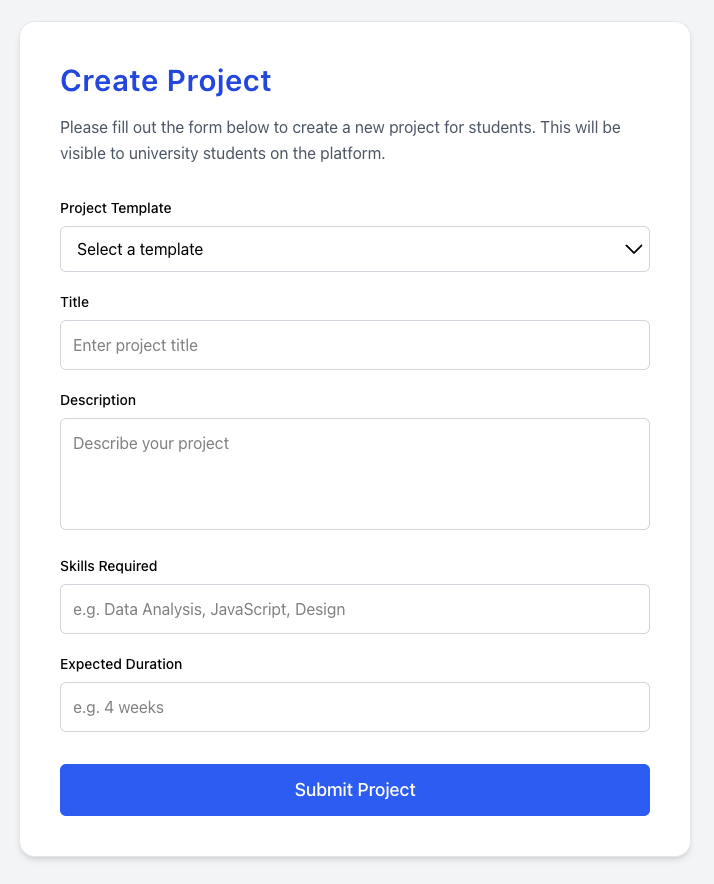
\includegraphics[width=0.85\linewidth]{figures/Organisation-generate-project.png}
  \caption{Organisation project wizard mock up that operationalises the toolkit entries.}
  \label{fig:project-creation}
\end{figure}
